\documentclass[conference]{IEEEtran}
\usepackage{amsfonts}
%\usepackage{amsthm}
\usepackage{graphicx}
\usepackage{fancyhdr}
\usepackage{floatflt}


\setlength{\parindent}{3em} \setlength{\oddsidemargin}{0in}
\setlength{\textwidth}{6.5in} % sets 1in left and right margins
\setlength{\topmargin}{0.20in} % change to 0.2in for regular latex
%\setlength{\headheight}{0in}
%\setlength{\footheight}{0.5in}
\setlength{\footskip}{0.5in}
\setlength{\textheight}{9.0in} %sets 1in top and bottom margins
\renewcommand{\baselinestretch}{1} %set to 1.5 for double spacing.

\newcommand{\br}{{\mathbf r}}
\newcommand{\bA}{{\mathbf A}}
\newcommand{\ba}{{\bf a}}
\newcommand{\bb}{{\bf b}}
\newcommand{\bc}{{\bf c}}
\newcommand{\bC}{{\bf C}}
\newcommand{\bg}{{\bf g}}
\newcommand{\bG}{{\bf G}}
\newcommand{\bd}{{\bf d}}
\newcommand{\be}{{\bf e}}
\newcommand{\bq}{{\bf q}}
\newcommand{\bs}{{\bf s}}
\newcommand{\bm}{{\bf m}}
\newcommand{\bn}{{\bf n}}
\newcommand{\bu}{{\bf u}}
\newcommand{\bv}{{\bf v}}
\newcommand{\bw}{{\bf w}}
\newcommand{\bx}{{\bf x}}
\newcommand{\by}{{\bf y}}
\newcommand{\bz}{{\bf z}}
\newcommand{\bbf}{{\bf f}}
\newcommand{\bE}{{\bf E}}
\newcommand{\bF}{{\bf F}}
\newcommand{\bL}{{\bf L}}
\newcommand{\bM}{{\bf M}}
\newcommand{\bN}{{\bf N}}
\newcommand{\bS}{{\bf S}}
\newcommand{\bT}{{\bf T}}
\newcommand{\bD}{{\bf D}}
\newcommand{\bX}{{\bf X}}
\newcommand{\bP}{{\bf P}}
\newcommand{\bQ}{{\bf Q}}
\newcommand{\bI}{{\bf I}}
\newcommand{\bR}{{\bf R}}
\newcommand{\bU}{{\bf U}}
\newcommand{\bV}{{\bf V}}
\newcommand{\bW}{{\bf W}}
\newcommand{\bY}{{\bf Y}}
\newcommand{\bZ}{{\bf Z}}
\newcommand{\bJ}{{\bf J}}
\newcommand{\bB}{{\bf B}}
\newcommand{\bzero}{{\bf 0}}
\newcommand{\bgamma}{{\mbox {\boldmath $\gamma$}}}
\newcommand{\btheta}{{\mbox {\boldmath $\theta$}}}
\newcommand{\bLambda}{{\mbox {\boldmath $\Lambda$}}}
\newcommand{\bPsi}{{\mbox {\boldmath $\Psi$}}}
\newcommand{\bPhi}{{\mbox {\boldmath $\Phi$}}}
\newcommand{\bphi}{{\mbox {\boldmath $\phi$}}}
\newcommand{\bcA}{{\mbox {\boldmath ${\cal A}$}}}
\newcommand{\bcB}{{\mbox {\boldmath ${\cal B}$}}}
\newcommand{\bcC}{{\mbox {\boldmath ${\cal C}$}}}
\newcommand{\bcD}{{\mbox {\boldmath ${\cal D}$}}}
\newcommand{\bcF}{{\mbox {\boldmath ${\cal F}$}}}
\newcommand{\bcN}{{\mbox {\boldmath ${\cal N}$}}}
\newcommand{\bcR}{{\mbox {\boldmath ${\cal R}$}}}
\newcommand{\bcS}{{\mbox {\boldmath ${\cal S}$}}}
\newcommand{\bcH}{{\mbox {\boldmath ${\cal H}$}}}
\newcommand{\bcI}{{\mbox {\boldmath ${\cal I}$}}}

\begin{document}

\title{Blind Multiuser Receiver Design}
%\author{Shu Wang and James Caffery, Jr.}

\author{\authorblockN{Shu Wang}
\authorblockA{LGE Mobile Research\\
San Diego, CA 92131-1807\\
\em Email: swang@lge.com} \and
\authorblockN{James Caffery, Jr.}
\authorblockA{University of Cincinnati\\
Cincinnati, OH 45221-0030\\
\em Email: jcaffery@ececs.uc.edu}}

\date{}
\maketitle
\begin{abstract}\small
The multiuser signal model not only helps us understand signal
structures but also plays a key role in multiuser receiver design.
In this paper, we present an alternative multiuser signal model
and discuss its applications for blind multiuser receiver design.
At first, we compare it with the conventional signal model and
signal subspace based signal model as well as their applications
in receiver design. The geometric interpretation, bit-error rate,
signal processing bounds, etc. of these signal models and blind
receivers are compared and discussed after that. Through these,
the trade-offs between the complexity and performance of blind
multiuser receiver design can be revealed. Computer simulations
are finally provided to demonstrate the performance and theoretic
analysis.
\end{abstract}

\section{Introduction}
Multiuser detection (MUD) is the strategy for mitigating multiple
access interference (MAI) effects and solving the near-far problem
with exploiting interference structure. MUD has been extensively
investigated over the past several years since MAI is the dominant
impairment for CDMA systems and even exists in the systems with
perfect power control~\cite{Verd98} and it is believed to be one
of the critical techniques for mitigating MAI effects and enabling
the high reliability and throughput of next-generation mobile
communication systems~\cite{Andr05}. Most recent research on MUD
has been devoted to blind detection and subspace-based signature
waveform or channel estimation for reducing the computation
complexity and prior
knowledge~\cite{Honi95,Torl97,Wang98,Zhang02,Wang03d,Wang05A,Wang05B}.
Blind multiuser receivers can achieve good performance with the
knowledge of only desired user's timing and signature waveform.
This assumption also is much closer to practical applications
where most interferences are unknown beforehand. However, most
existing blind receivers are known to be too complicated for
high-data-rate applications.

In the procedure of advanced multiuser receiver development, it is
known that a proper received signal model can help us understand
received signals as well as receiver design. There are two popular
multiuser signal models which have been intensively discussed for
multiuser receiver design. They are the conventional multiuser
signal model and the subspace-based multiuser signal model. In the
conventional signal model, each received signal is directly taken
as a linear combination of actual signal
signatures~\cite{Verd98,Honi95,Zhang02}. Most related blind
multiuser receivers are developed either by explicitly estimating
the signal signature~\cite{Torl97} or by removing interfering
signal components using adaptive filtering techniques, e.g., the
blind receiver design with Wiener filter~\cite{Honi95} and Kalman
filter~\cite{Zhang02} techniques. Though the conventional signal
model provides us a natural view of received signals, the involved
signature waveforms or amplitudes information is unknown and it
usually take the receiver lots of efforts to obtain it before
detection. For compensating the weakness of the conventional
signal model, the subspace signal model is proposed with
subspace-based signal processing techniques~\cite{Wang98}. In the
subspace signal model, each received signal is taken as a linear
combination of signal subspace bases, which can be obtained by
subspace signal processing techniques on the autocorrelation
matrix of received signals. Subspace signal mode can be taken as a
result of parametric signal modelling and provides a in-depth
comprehension of received signals. Though subspace-based
approaches don't need explicitly estimate each user's signal
signature and the initialization and adaptive speed are improved
with good performance, the signal subspace formation procedure
still is not trivial.

It is known that the conventional signal model provides us the
foundation for both optimal and conventional multiuser receiver
design and subspace signal model helps us understand signal
underneath structure. However, neither of them is easy enough for
developing the blind multiuser receivers for high-speed CDMA
systems~\cite{Andr05}. In order to solve the near-far problem with
minimum prior knowledge and computation complexity, we propose a
new blind multiuser model with directly connecting the current
received signal and several previous received signal while no
explicitly signal structure estimation. With this blind signal
model and widely employed signal estimation criteria including
least squares (LS), minimum mean-squared errors (MMSE) and maximum
likelihood (ML), several noval blind multiuser receivers are
developed. There is no statistical signal estimation or subspace
separation procedure required. Only a minimum number of previously
received signals and the desired user's signal signature waveform
and timing are required. Hence the computation complexity and
detection delay can be much reduced. After this, we compare the
proposed blind signal model and receivers with the conventional
signal model and subspace signal mode and their blind receivers.
The trade-off between the performance and complexity in blind
receiver development is discussed too. Computer simulations are
finally provided.

\section{Multiuser Signal Models}
The forward-link transmissions in a single-cell DS/CDMA system
with $K$ active users is discussed here. The channel is multiplath
channel with $P$ strong paths~\footnote{Strong paths are those to
be explicitly combined by RAKE receiver.} and corrupted by
additive white Gaussian noise (AWGN). The baseband representation
of the received signal due to user $k$ is given by
\begin{equation}
\begin{array}{l}\hspace{-0.2in}
r_k(t)=\sum\limits_{p=1}^{P}\alpha_{pk}A_k[n]
b_k[n]c_k(t-nT-\tau_p)+n_k(t)
\end{array}
\end{equation}
\noindent where $\alpha_{pk}$ is the $p$th path loss of user $k$'s
signal, $b_k{[n]}$ is the $n$th bit sent by user $k$. We assume
that the $\left\{b_k{[n]}\right\}$ are independent and identically
distributed random variables with $E\left\{b_k{[i]}\right\}=0$ and
$E\left\{|b_k{[i]}|^2\right\}=1$. The parameters $c_k(t)$ denote
the normalized spreading signal waveform of user $k$ during the
interval $[0,\ T]$, $0\leq\tau_1\leq\tau_2\leq\ldots\leq\tau_P$,
denotes $P$ different transmission delays from the base station to
user $k$ and $A_k[n]$ is the received signal amplitude for user
$k$ at time $t=nT$, which depends on the possible channel
statistics. The total baseband signal received by user $k$ is
\begin{equation}
\begin{array}{rcl}
\tilde{r}(t)&=&\sum\limits_{k=1}^{K}r_k(t)
\end{array}
\end{equation}
The received signal $\tilde{r}(t)$ is passed through the
corresponding chip matched filter (CMF), $\phi(t)$, and RAKE
combiner. The combined output $r(t)$ is~\footnote{Without loss of
the generality, we drop the time index $n$ in the following
discussion.}
\begin{equation}\hspace{-0.0in}
\begin{array}{rcl}
r(t)&=&A_k b_k c_k(t-nT-\tau_1)\otimes \phi(t-\tau_1)+ \\
&&\hspace{0.0in} m_{\rm ISI}(t) + m_{\rm MAI}(t) + n(t)
\end{array}\label{r_t}
\end{equation}
\noindent where
\begin{equation} \hspace{-0.05in}
\begin{array}{rcl}
 m_{\rm ISI}(t)&=&\\
 &&\hspace{-0.83in}\sum\limits^{P}_{p\neq
q}\beta_{qk} \alpha_{pk}A_kb_kc_k(t-nT+\tau_{q1}-\tau_1)\otimes
\phi(t-\tau_1)
\end{array}
\end{equation}
\noindent is the intersymbol interference (ISI) to user $k$,
\begin{equation} \hspace{-0.17in}
\begin{array}{rcl}
m_{\rm MAI}(t)&=&\sum\limits_{i\neq
 k}^{K}A_ib_ic_i(t-nT-\tau_1)\otimes\phi(t-\tau_1)+\\
 &&\hspace{-0.75in}\sum\limits_{i\neq
 k}^{K}\sum\limits^{P}_{p\neq
q}\beta_{qk}
\alpha_{pi}A_ib_ic_i(t-nT+\tau_{q1}-\tau_p)\otimes\phi(t-\tau_1)
\end{array}
\end{equation}
\noindent is the MAI to user $k$, $\beta_{qk}$ is the weight of
the $q$th RAKE finger with
$\sum\limits_{q=1}^{P}\beta_{qk}\alpha_{qk}=1$ and $\tau_{q1} =
\tau_{q}-\tau_1$ is the propagation delay difference between the
$1$st path and $p$th path. $\otimes$ denotes the convolutional
product. $n(t)$ is AWGN with variance $\sigma^2$. Because of
$m_{\rm MAI}(t)$ existing in the received signal $r(t)$, the
performance of conventional matched filter receiver suffers from
the so-called near-far problem~\cite{Verd98}. Multiuser detection
is one of the receiver techniques for solving this problem.

\subsection{Conventional Signal Model}
After RAKE combining, the user $1$'s output can be sampled at
$f_s=1/T_s$ and directly expressed by~\footnote{Without loss of
the generality, we name the first user as the desired user.}
\begin{equation}\hspace{-0.1in}
\begin{array}{rcl}
\br&=&\left[
\matrix{r(nT+T_s+\tau_1)&\ldots&r(nT+LT_s+\tau_1)}\right]^{\rm
T}\\
 &=&\sum\limits_{k=1}^{K} A_k b_k \bs_k + \bn \\
 &=&\bS \bA \bb + \bn
\end{array}\label{r_sync}
\end{equation}
\noindent where $\bS=[\bs_1\ \bs_2\ \ldots\ \bs_K]$ is the
received spreading signature matrix combined with inter-chip
interference (ICI), inter-symbol interference (ISI) and MAI
information, and $L=T/T_s$ is the number of samples per symbol,
which should not be less than the spreading gain $L_c$. Most MUD
schemes including optimum and conventional MUD are developed from
(\ref{r_sync}), which is named conventional multiuser signal
model. They are well documented in~\cite{Verd98}. One of the major
problems using (\ref{r_sync}) is $\left\{\bs_k,\
A_k:k\neq1\right\}$ or possible timing is unknown at receiver.
This may make multiuser receiver design complicated.

\subsection{Subspace Signal Model}
It is known that it is hard to accurately estimate the
$\left\{\bs_k:k\neq1\right\}$ in (\ref{r_sync}) in order to
directly apply the well-developed optimum or conventional
multiuser detection schemes. Another approach is to use
subspace-based signal model and signal processing techniques for
reconstruct the conventional detectors~\cite{Wang98}. In the
subspace signal model, $\br$ is modelled by the combination of the
signal subspace bases $\left\{\bu_{sk}:1\leq k\leq K\right\}$:
\begin{equation}
\begin{array}{rcl}
\br&=&\bU_{s}\bphi+\bn
\end{array}\label{r_ss}
\end{equation}
\noindent where $\bU_{s}=\left[\bu_{s1}\ \bu_{s2}\ \ldots\
\bu_{sK}\right]$, $\bphi$ is a vector defined by
\begin{equation}
\begin{array}{rcl}
\bphi&=&\bPhi\bA\bb
\end{array}
\end{equation}
\noindent with $\bPhi$ is a $K\times K$ matrix. The original
signal signature matrix $\bS$ can now be expressed by
\begin{equation}
\begin{array}{rcl}
\bS&=&\bU_{s}\bPhi
\end{array}.
\end{equation}
\noindent One of the major advantages of the subspace signal model
(\ref{r_ss}) is that the signal subspace bases
$\left\{\bu_{sk}:1\leq k\leq K\right\}$ are much easier to be
estimated than the actual signal signature waveforms so that the
blind receiver design can be much simplified. These signal bases
can be estimated applying subspace decomposition on the
autocorrelation matrix $\bR$:
\begin{equation}
\begin{array}{rcl}
\bR &=&{\rm E}\{\br\br^{\rm T}\}\\
&=&\left[\matrix{\bU_{s}&\bU_{n}}\right]\left[\matrix{\bLambda_{s}&\cr&\bLambda_{n}}\right]\left[\matrix{\bU_{s}^{\rm
T}\cr\bU_{n}^{\rm T}}\right]
\end{array}.\label{R}
\end{equation}
\noindent where $\bU_{n}$ denotes the noise subspace bases and
$\left[\cdot\right]^{\rm T}$ denotes the transportation operation.

\subsection{The Proposed Blind Signal Model}
As we can see, one of the difficulties in using the conventional
signal model or subspace signal model for blind receiver design is
the signal signatures $\left\{\bs_k:k\neq1\right\}$ in
(\ref{r_sync}) or the signal subspace matrix $\bU_{s}$ in
(\ref{r_ss}) are unknown beforehand. Instead we propose a known
blind signature matrix $\bcS$
\begin{equation}
\begin{array}{rcl}
\bcS&=&[\matrix{\bs_1&{\br}_{1}&{\br}_{2}&\ldots&{\br}_{M-1}}]\\
&=&\bS\bD + {\bN}
\end{array} \label{S_0}
\end{equation}
\noindent where $\left\{\br_{m}:1\leq m\leq M-1\right\}$ are
previously received and detected signal vectors and
\begin{equation}\hspace{-0.0in}
\begin{array}{c}
 \bD=\left[\matrix{1 & \bar\bd^{\rm T}\cr\bzero&\tilde\bD }\right]=\left[\matrix{\be & \matrix{\bar\bd^{\rm T}\cr \tilde{\bD}} }\right]
  =\left[\matrix{\bg^{\rm T} \cr \matrix{\mathbf{0}& \tilde{\bD}}
 }\right]
\end{array}\label{D}
\end{equation}
\noindent is the $K\times M$ data matrix associated with $\bcS$.
Now the received signal can be expressed by
\begin{equation}
\begin{array}{rcl}
\br&=&\bcS\bbf + \tilde{\bn} \label{r_blind}
\end{array}
\end{equation}
\noindent with the $M \times 1$ vector $\bbf$ defined by
\begin{equation}
\begin{array}{rcl}
\bbf&=&\bD^{+}\bA\bb
\end{array}, \label{DetectorVector}
\end{equation}
\noindent where $\tilde{\bn}$ is the new $L\times 1$ AWGN vector
defined by
\begin{equation}
\begin{array}{rcl}
\tilde{\bn}&=&\bn-{\bN}\bD^{+}\bA\bb
\end{array} \label{new_noise}
\end{equation}
\noindent $\be=[\matrix{1&\bzero}]^{\rm T}$ is a vector of length
$K$, $\bg = \left[\matrix{1&\bar\bd}\right]^{\rm T}$ is a vector
of length $M$.

Different to the models in (\ref{r_sync}) and (\ref{r_ss}), the
key component $\bcS$ in (\ref{r_blind}) is known beforehand. This
makes this model ready for designing new blind multiuser receivers
from the beginning. After we estimate $\bbf$ with conventional
signal estimation techniques, the detection of user $1$'s
information can easily be done with knowing $d_1=A_1b_1$, which
can be estimated by
\begin{equation}
\begin{array}{rcl}
\hat{d}_{1} &=&\bg^{\rm T}\bbf
\end{array}.\label{d_1}
\end{equation}

\section{Blind Multiuser Receiver}
In the conventional blind multiuser receiver design, adaptive
filtering techniques are employed for removing noise and
interference. Statistical signal spectrum analysis techniques are
used in subspace-based blind multiuser receiver design. With the
proposed blind multiuser signal model (\ref{r_blind}), we use
conventional multiuser detection techniques for blind receiver
design.

\subsection{Conventional Blind Multiuser Detection}
With the conventional signal model in (\ref{r_sync}), there are
two popular directions for designing blind multiuser receivers.
One is to estimate the unknown $K-1$ signal signatures
$\left\{\bs_k:k\neq1\right\}$ and then apply known
optimal/conventional detectors on $\br$. This approach is know to
be computation-intensive since the signal waveform estimation
itself is not simple~\cite{Torl97}. The other one is to use
adaptive filter techniques with some signal processing criteria.
Under this direction, there are well-known minimum output energy
(MOE) detector, blind MMSE detector and blind Kalman
detector~\cite{Honi95,Verd98,Zhang02}. However, these blind
detectors are known to be slow in their adaptive procedures.

\subsection{Subspace-Based Blind Multiuser Detection}
With the subspace signal mode in (\ref{r_ss}), the first step
usually is to separate signal/noise subspaces and estimate
$\bU_{s}$ using (\ref{R}). After this, the least-square-based
decorrelating detector is given by~\cite{Wang98}
\begin{equation}\hspace{-0.05in}
\begin{array}{l}
\bd_{\rm DD1}=\frac{1}{\bs_1^{\rm
T}\bU_{s}\left(\bLambda_{s}-\sigma\bI\right)^{-1}\bU_{s}^{\rm
T}\bs_{1}}\bs_{1}^{\rm
T}\bU_{s}\left(\bLambda_{s}-\sigma\bI\right)^{-1}\bU_{s}^{\rm
T}\br
\end{array}
\end{equation}
\noindent and the MMSE detector can be expressed by
\begin{equation}
\begin{array}{rcl}
\bd_{\rm MMSE1}&=&\frac{1}{\bs_1^{\rm
T}\bU_{s}\bLambda_{s}^{-1}\bU_{s}^{\rm T}\bs_{1}}\bs_{1}^{\rm
T}\bU_{s}\bLambda_{s}^{-1}\bU_{s}^{\rm T}\br
\end{array}
\end{equation}

\subsection{New Blind Multiuser Detection Approaches}
It shows that one of the key components in the proposed blind
receiver design framework is the estimation of $\bbf$. After this
$\bd_1$ can be estimated with (\ref{d_1}).

With the blind signal model in (\ref{r_blind}), one possible
approach is firstly to estimate the detection vector $\bbf$.
Obviously different signal estimation criteria may lead to
different solutions. If the LS criterion is direct applied here,
the traditional LS estimation of $\bbf$ can be expressed by
\begin{equation}
\begin{array}{rcccl}
{\bbf}_{\rm
LS}&=&\matrix{\mbox{arg}\min\limits_{\bx}\left\|\br-\bcS\bx\right\|_2}&=&\bcS^+\br
\end{array}
\label{LSProb}
\end{equation}
\noindent with the assumption that $\bcS$ is error-free.

If $\bcS$ is assumed to be error-polluted in the above LS
estimation problem (\ref{LSProb}), we have the total least squares
(TLS) problem
\begin{equation}
\begin{array}{l}
\left[\matrix{\bcS_{\rm TLS}\cr\bbf_{\rm
TLS}}\right]=\matrix{\mbox{arg}\min\limits_{\bar{\bcS},\
\bx}\left\|\left[ \matrix{\bcS\cr\br} \right] - \left[
\matrix{\bar{\bcS}\cr\bar{\bcS}\bx}\right]\right\|_2}
\end{array}.
\label{TLSProb}
\end{equation}
\noindent With solving (\ref{TLSProb}), the TLS estimation of
$\bbf$ can be written by
\begin{equation}
\bbf_{\rm TLS} = \left(\bcS^{\rm
T}\bcS-\sigma_{K+1}^2\bI\right)^{-1}\bcS^{\rm T}\br\ ,
\end{equation}
\noindent where $\sigma_{K+1}$ is the $K+1$th smallest singular
value of $\left[\bcS\ \br\right]$ and is assumed to be not greater
than the $k$th largest singular value of $\bcS$.

If only the first column of the $\bcS$ in (\ref{LSProb}) is
assumed to be error-free, we have the mixed least-square (MLS)
problem:
\begin{equation}
\begin{array}{l}
\left[\matrix{\bcS_{\rm MLS}\cr\bbf_{\rm
MLS}}\right]=\matrix{\mbox{arg}\min\limits_{\bar{\bcS},\
\bx}\left\|\left[\matrix{\tilde{\bcS}\cr\br}\right]-\left[\matrix{\bar{\bcS}\cr[\bs_1\
 \bar{\bcS}]\bx}\right]\right\|_{2} }
\end{array},\label{MLSProb}
\end{equation}
\noindent With solving (\ref{MLSProb}), the MLS estimation of
$\bbf$ can be written by
\begin{equation}\hspace{-0.09in}
\begin{array}{rcl}
\bbf_{\rm MLS}&=&\left(\bcS^{\rm
T}\bcS-\sigma^2\left[\matrix{\bzero&\mathbf{0}\cr\mathbf{0}&\mathbf{I}_{M-G}}\right]\right)^{-1}\bcS^{\rm
T}\br
\end{array},
\end{equation}
\noindent where $\sigma$ is the smallest singular value of
$\left[\bcS\ \br\right]$.

If the minimum variance unbiased (MVU) criterion is applied,
$\bbf$ can be estimated by
\begin{equation}
\begin{array}{rcl}
{\bbf}_{\rm MVU}&=&\left(\bcS^{\rm
T}\bR_{\tilde{\bn}}^{-1}\bcS\right)^{-1}\bcS^{\rm
T}\bR_{\tilde{\bn}}^{-1}\br
\end{array}. \label{MVU}
\end{equation}
\noindent where
$\bR_{\tilde{\bn}}=\mbox{E}\left\{\tilde{\bn}\tilde{\bn}^{\rm
T}\right\}$ denotes the autocorrelation matrix of $\tilde{\bn}$.

If the MMSE criteria is applied, $\bbf$ can be estimated by
\begin{equation}\hspace{-0.07in}
\begin{array}{rcl}
{\bbf}_{\rm MMSE}&=&\mbox{arg}\min\limits_{\hat{\bbf}}\mbox{E}\|\hat{\bbf}-\bbf\|_2^2\\
&=&\left(\bR_{\bbf}^{-1}+\bcS^{\rm
T}\bR_{\tilde{\bn}}^{-1}\bcS\right)^{-1}\bcS^{\rm
T}\bR_{\tilde{\bn}}^{-1}\br
\end{array}. \label{MSE}
\end{equation}

\section{Performance Analysis and Comparison}

\subsection{Comparison with Existing Blind Detectors}
\begin{figure*}[t]\label{SchemComp}\small
\center{Table 1. The comparison of the proposed framework and
other detection approaches}
\begin{center}
\begin{tabular}{lccccc}
Parameters & Conv. MUD & Conv. IC &Blind MMSE & Subspace Approaches & Blind MUD\\
\hline \hline
Signature of desired user(s) & $\bf\Box$ & $\bf\Box$ & $\mathbf\Box$ &  $\mathbf\Box$ & $\mathbf\Box$ \\
Signature of other users & $\mathbf\Box$ & $\bf\Box$ & & &  \\
Timing of desired user(s)  & $\mathbf\Box$ & $\bf\Box$ & $\mathbf\Box$ & $\mathbf\Box$ & $\mathbf\Box$ \\
Timing of other users  & $\mathbf\Box$ & $\bf\Box$ & & & \\
Received amplitudes  & $\mathbf\Box$ & $\bf\Box$ & &  &\\
ECC decoding-integratable& $\mathbf\Box$ &$\bf\Box$ & && $\mathbf\Box$ \\
Initialization~{\small *} &  & & $\ge L$ & $\ge L$ & $M$\\
Latency & $1$ & $K-1$& $1$ & $1$ & $1$ \\
Complexity order & $1$ & $K$ & $1$ & $1$ & $1$ \\
\hline \hline \multicolumn{5}{l}{\tiny * For blind MMSE or
subspace approaches, they typically require much more than $L$
signals before their first detection.}
\end{tabular}
\end{center}
\end{figure*}
The comparison between the proposed framework and other major
schemes is presented in Table~1. The proposed framework only
requires $M$, where $L\ge M\ge (K-G)$, previous received signal
for signal detection and its complexity is closed to conventional
detectors while other blind approaches typically requires a lots
more than $L$ signals~\cite{Madh94,Wang98,Zhang02}.

\subsection{Geometrical Interpretation} It is known that
conventional decorrelating detector can be interpolated as an
oblique projection of $\bs_1$ onto the orthogonal complement of
the signal subspace $\bar\mathbb{S}_{1}=\mbox{span}\left\{\bs_k :
k=2,\ 3,\ \ldots ,\ K\right\}$ along the orthogonal complement of
$\mathbb{S}_{1}=\mbox{span}\left\{\bs_1\right\}$~\cite{Elda02}
while conventional or blind MMSE detection can be taken as a
balance between single-user matched filter and decorrelating
detector. Subspace-based decorrelating detector and MMSE detector
have the same geometrical interpretation with the conventional
detectors, respectively.

In the proposed blind least-square receiver, the projection using
$\bcS$ can be interpreted as an oblique projection of $\bs_1$ onto
the orthogonal complement of the signal subspace
$\tilde\mathbb{S}_{1}=\mbox{span}\left\{\br_m : k=1,\ 2,\ \ldots
,\ M-1\right\}$, instead of $\bar\mathbb{S}_{1}$, along the
orthogonal complement of $\mathbb{S}_{1}$. Since
$\tilde\mathbb{S}_{1}\neq\bar\mathbb{S}_{1}$, there is some
deviation between this projection and the previous one using
$\bar\mathbb{S}_{1}$ and there is a difference between $d_1$ and
the first element of $\bbf$. Fortunately, this difference can be
compensated with (\ref{d_1}).

\subsection{Noise Enhancement} It is known that there is a noise
enhancement issue in the LS-based conventional decorrelating
detection. With conventional decorrelating detection, the output
signal-to-noise ratio (SNR) for user $k$ is decreased by
$\left[\bR_{\bs}^{+}\right]_{kk}^{-1}$. With the proposed blind LS
multiuser receiver, there is another noise enhancement issue.
Following Girko's law, providing $\alpha=\frac{K-1}{M}$ is fixed,
the diagonal element of
$\frac{1}{M}\left(\bD^{+}\bb\right)\left(\bD^{+}\bb\right)^{\rm
T}$ can be approximated to be $1-\alpha$ with $K$, $M$
$\rightarrow\infty$~\cite{Muller}. And the autocorrelation matrix
of $\tilde\bn$ can be expressed by
\begin{equation}
\begin{array}{rcl}
\bR_{\tilde\bn}&=&\frac{2M+K-1}{M}\sigma^{2}\bI
\end{array}.\label{noise_var_new}
\end{equation}
\noindent It shows that the noise variance is increased by
$\frac{2M+K-1}{M}$.
\subsection{Cram\'{e}r-Rao Lower Bound} The Cram\'{e}r-Rao lower
bound (CRLB) is given by the inverse of the Fisher information
matrix (FIM). For the conventional signal model, CRLB of
$\bd=\bA\bb$ estimation is given by
\begin{equation}
\begin{array}{rcl}
{\rm CRLB}(\bd\ |\ \bS)&=&\sigma^{2}\left(\bS^{\rm
T}\bS\right)^{\rm -1}
\end{array}.\label{CRLB_b}
\end{equation}
\noindent It shows that the conventional decorrelating detection
can achieve maximum likelihood sense if the amplitude $\bA$ is
unknown. For the blind signal model, if the blind spreading matrix
$\bcS$ is known beforehand, we first define the parameter vector
$\mathbf{\psi} = \left[\tilde{\sigma}^{2}\ \bbf^{\rm
T}\right]^{\rm T}$, where $\tilde{\sigma}^{2}
=(1+\frac{M-1}{M-K})\sigma^{2}$, for computing the FIM
\begin{equation}
\begin{array}{rcl}
{\bI(\mathbf{\phi})} &=& {\rm E} \left\{ \left( \frac{\partial
\ln{\cal L}}{\partial \mathbf{\psi}} \right) \left( \frac{\partial
\ln{\cal L}}{\partial \mathbf{\psi}} \right)^{\rm T} \right\}
\label{fim}
\end{array}
\end{equation}
\noindent where $\ln{\cal L}$ is the log-likelihood function given
by
\begin{equation}
\begin{array}{rcl}
\ln{\cal
L}&=&C-L\ln\tilde{\sigma}^2-\frac{1}{2\tilde{\sigma}^2}\parallel\mathbf{e}\parallel_2^2
\end{array},\label{logl}
\end{equation}
\noindent $C$ is a constant and $\mathbf{e}=\br-\bcS\bbf$.
Providing $\bcS$ is known, the closed-form CRLB expression of
$\bbf$ is then given by
\begin{equation}
\begin{array}{rcl}
{\rm CRLB}(\bbf\ |\
\bcS)&=&(1+\frac{M-1}{M-K})\sigma^{2}(\bcS^{\rm T}\bcS)^{\rm +}
\end{array}.\label{CRLB_f}
\end{equation}
\noindent It shows that the accuracy of estimating $\bbf$ may
increase with increasing $M$.

\subsection{Bit-Error Rate}
With decorrelating detection and BPSK modulation, the bit-error
rate (BER) for user $k$ is
\begin{equation}
\begin{array}{rcl}
P_{ek,\rm\small DD} &=&
Q\left(\frac{A_{k}}{\sigma\left[\bR_{\bs}^{+}\right]_{kk}}\right)
\end{array}.\label{BER_DD}
\end{equation}
\noindent Similarly for the blind LS multiuser receiver, the
detection BER can be written by
\begin{equation}\hspace{-0.07in}
\begin{array}{rcl}
P_{e1,\rm\small LS} &=&
Q\left(\frac{\sqrt{\frac{M}{2M+K-1}}}{\left[\left(\bcS^{\rm
T}\bcS\right)^{+}\right]_{11}}\frac{A_k}{\sigma}\right)\ .
\end{array}\label{BER_LS}
\end{equation}

\subsection{Asymptotic Multiuser Efficiency}
A commonly used performance measure for a
multiuser detector is asymptotic multiuser efficiency (AME) and
near-far resistance~\cite{Verd98}. The AME of the conventional
decorrelating detection approach is
\begin{equation}
\begin{array}{rcl}
{\eta}_k&=&\left[\bR_{\bS}^{+}\right]_{kk}^{-1}
\end{array}
\end{equation}
\noindent and the AME of the proposed schemes is
\begin{equation}
\begin{array}{rcl}
\bar{\eta}_k&=&{\frac{M}{2M+K-1}}\left[\bR_{\tiny\bcS}^{+}\right]_{kk}^{-1}
\end{array}
\end{equation}
\noindent where $\bR_{\tiny\bcS}=\bcS^{\rm T}\bcS$ and
$\left[\cdot\right]_{kk}$ denotes the $k$th diagonal element of
the matrix.

\section{Computer Simulations}

\begin{figure} \center{
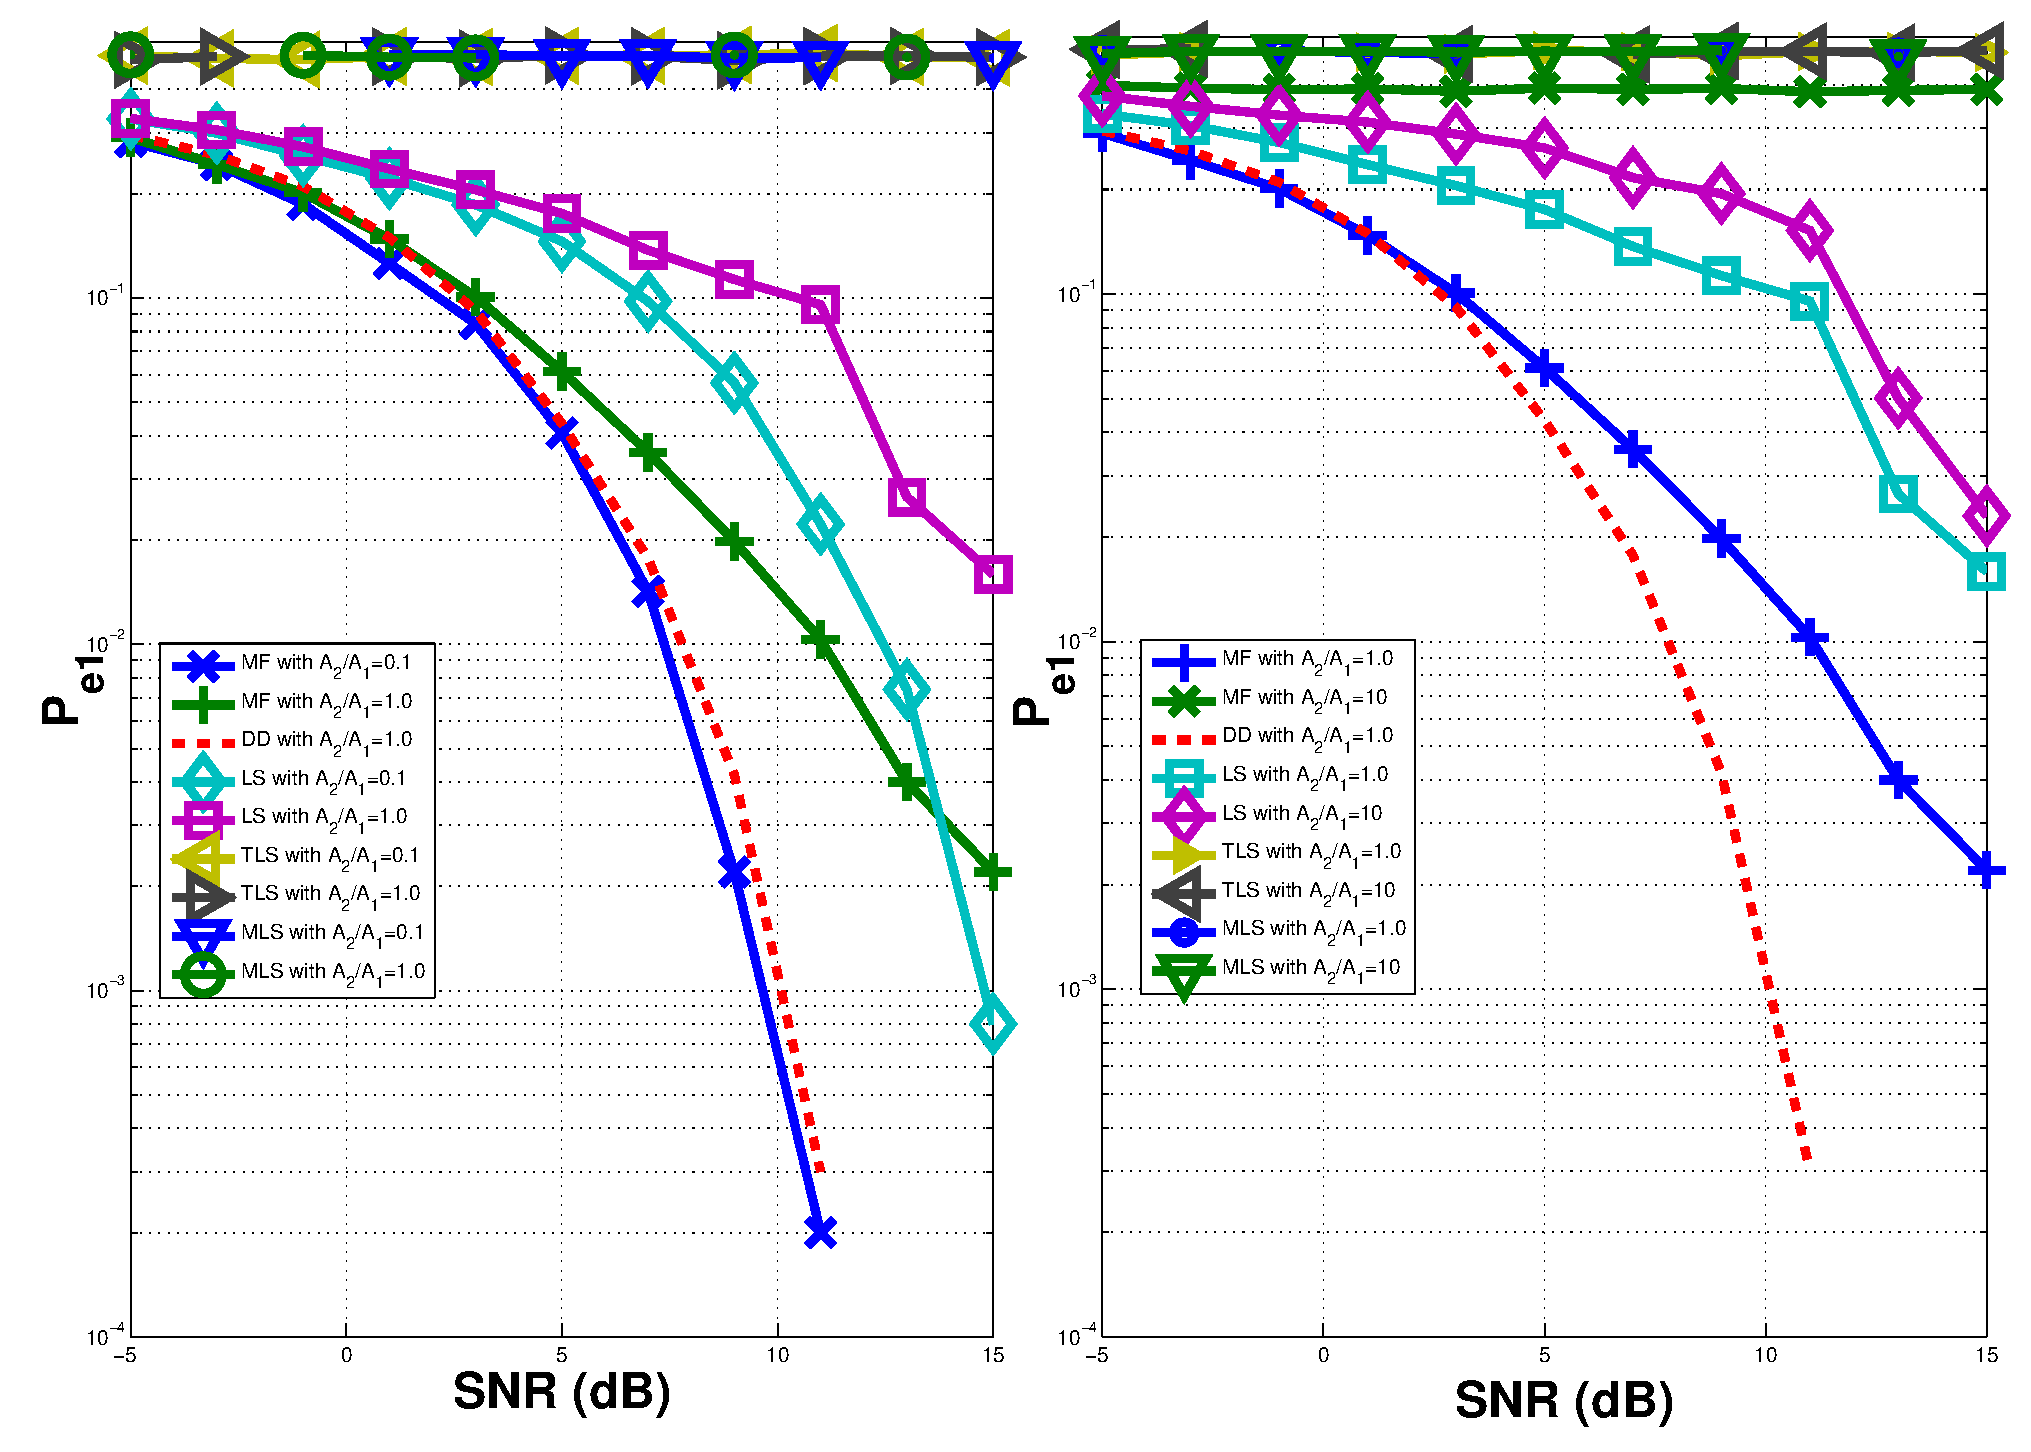
\includegraphics[width=3.2in]{BER_40_16_4.eps}
\caption{ The BER of various schemes against SNR. $K=16$, $M=40$
and $G=4$.} }\label{BER}
\end{figure}

Single-cell DS/CDMA synchronous multiuser system is simulated
here. The spreading sequence are random sequences with $L=64$. In
the simulations, previous amplitude estimation is used for the
next detection. In Fig 1, there are $16$ users and the group size
$G=3$ with $M$. From Subplot (a) in Fig. 1, it is interesting to
see that the performance of the simplest blind LS detector has the
best performance when SNR is greater than $14$dB. From Subplot
(b), it is very impressive to find that the performance of the
blind LS detector still is very good. In Fig. 2, there are two
active users simulated with $G=1$ and $M=40$. The crosscorrelation
between these two users is $\rho=0.28$. We can see that the
performance of proposed schemes is stable against the change of
the near-far ratio. However, due to the noise enhancement we
analyzed before, their performance is not as good as the
conventional decorrelating detector, which has the best near-far
resistance.

\begin{figure} \center{
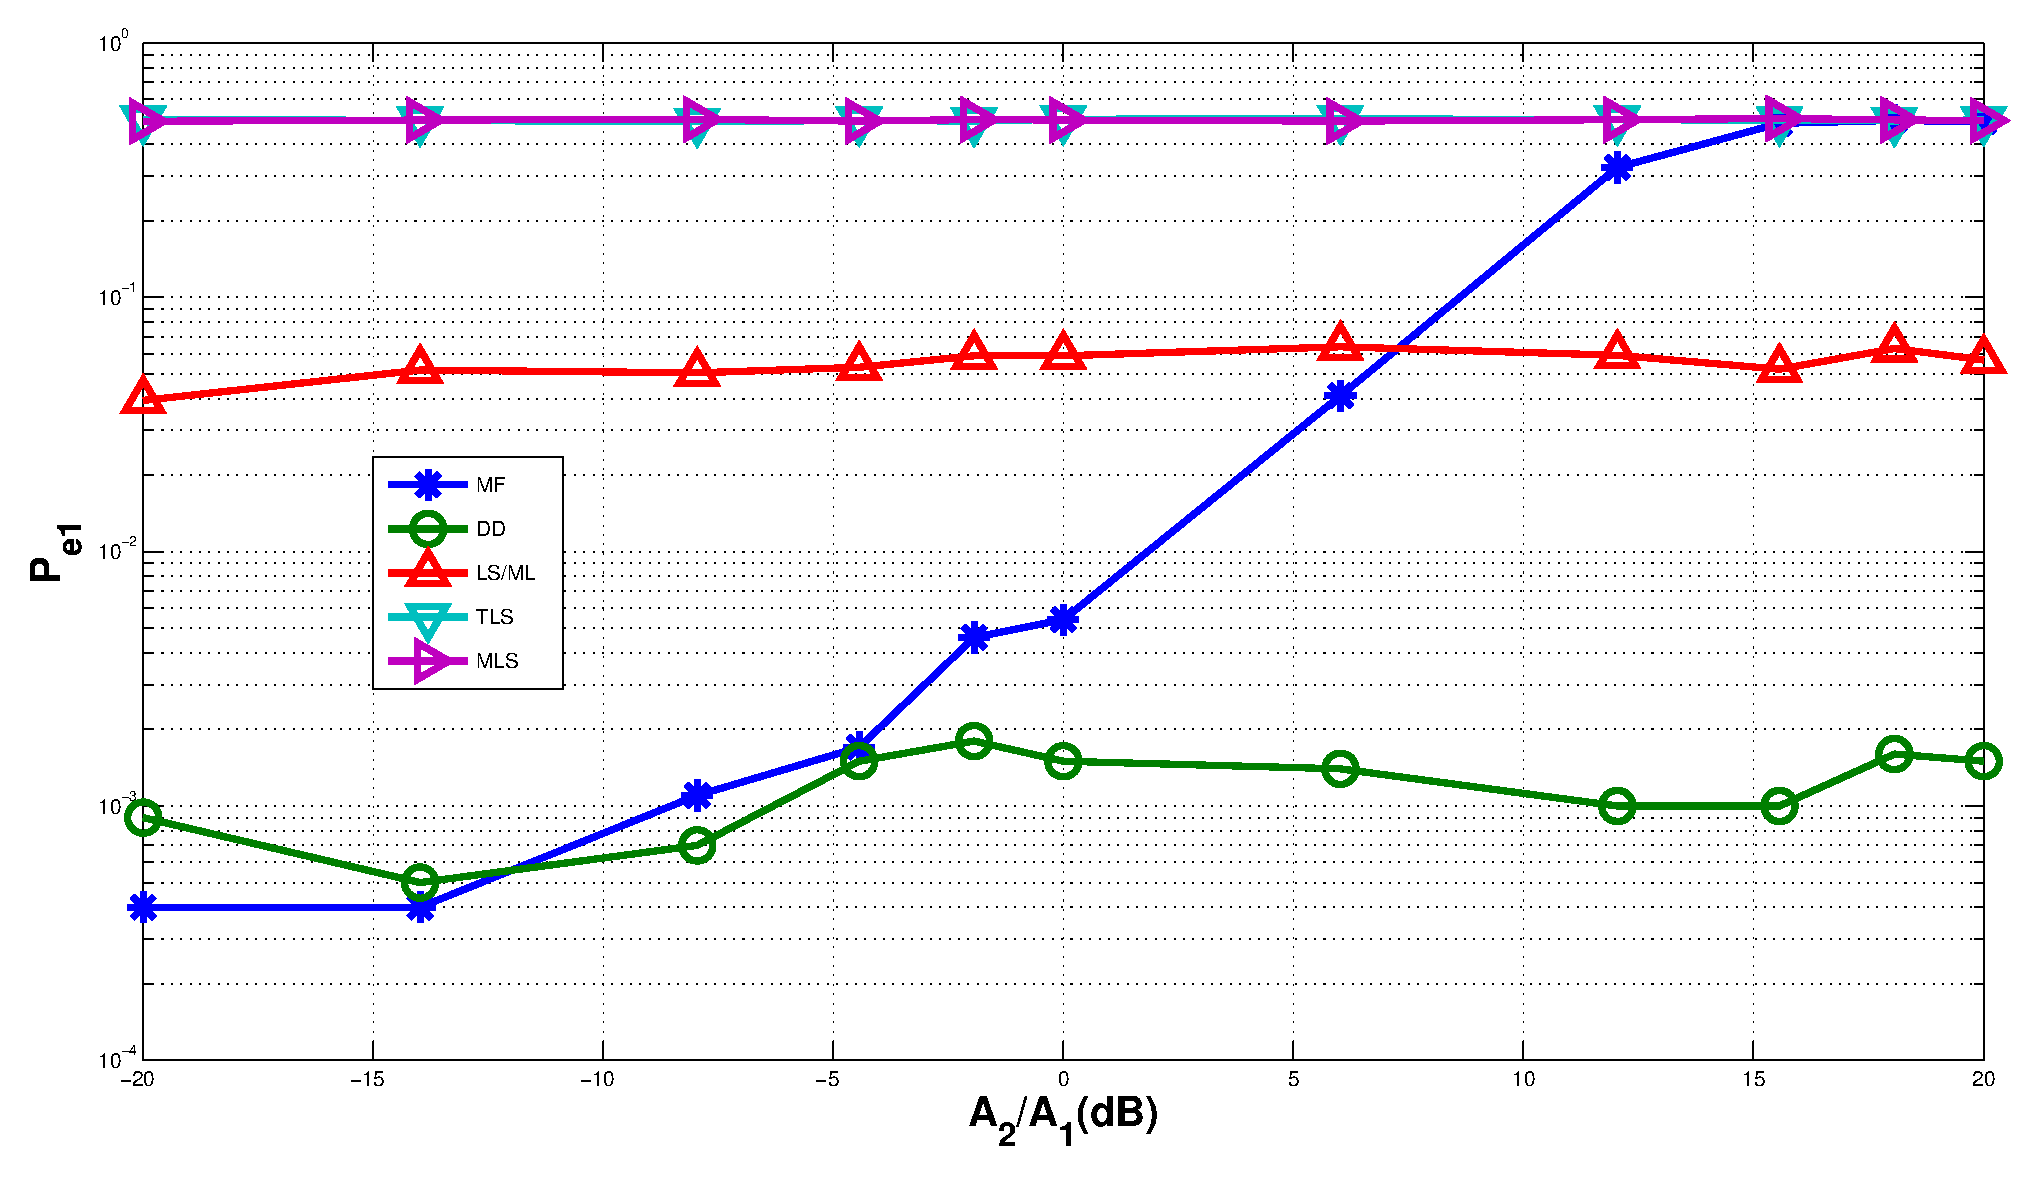
\includegraphics[width=3.2in]{NFR_028_10.eps}
\caption{ The near-far resistance of various schemes. ${\rm
SNR}=10{\rm dB}$, $\rho=0.28$, $M=40$ and $K=2$.} }\label{NFR}
\end{figure}

\section{Conclusions}
In this paper, we present a different approach for blind multiuser
receiver design and side-by-side compare it with the existing
conventional blind receiver and subspace-based receiver designs in
terms of geometric properties, asymptotic multiuser efficiency and
near-far resistance, noise enhancement, Cram\'{e}r-Rao lower
bound, etc., and discussed the trade-off between performance and
complexity.
%\small
\bibliographystyle{unsrt}
\bibliography{FastBDD,InterferenceCancellation}
\end{document}
